\documentclass[10pt,twocolumn,letterpaper]{article}

\usepackage{cvpr}
\usepackage{times}
\usepackage{epsfig}
\usepackage{graphicx}
\usepackage{amsmath}
\usepackage{amssymb}

% Include other packages here, before hyperref.
\usepackage[pagebackref=true,breaklinks=true,letterpaper=true,colorlinks,bookmarks=false]{hyperref}

% Pages are numbered in submission mode, and unnumbered in camera-ready
\ifcvprfinal\pagestyle{empty}\fi
\begin{document}

%%%%%%%%% TITLE
\title{Snakes: Static and Scale-Space Experiments}

\author{Konstantinos Katergaris\\
Arizona State University\\
1151 S Forest Ave, Tempe, AZ\\
{\tt\small kkaterga@asu.edu}}

%\thispagestyle{empty}

\maketitle
\begin{abstract}
This report implements an active contour model snakes on a synthetic image one without noise and the other with synthetic noise added. This synthetic image is of a white circle and a black background. The snake is initialized around the circle and then evolved based on internal and external energies later circling around the original circle. Results show that the snake algorithim is effective on find edges of objects in images.
\end{abstract}
\section{Overview}
The snakes model is a active contour model  used for image contour detection. It minimizes the following energy function: \[ E_{\text{snake}} = E_{\text{int}} + E_{\text{image}} + E_{\text{ext}},\], where $E_{\text{int}}$ is the internal energy which control the smoothness and elasticity of the contour,  $E_{\text{ext}}$ the external forces, attract the snake to salient features like edges, and $E_{\text{image}}$ is the image energy attracting the snake to object boundaries. The balance between these forces allows the snake to adapt to object boundaries dynamically. More information can be found on the specific details in the original paper\cite{kass1988snakes}

\section{Implementation}
The model was implemented using Python using NumPy for array operations and mathematical computations, and SciPy for image processing tasks like applying filters and computing image gradients. The snake, is represented as an array of points initialized around an object of in the image that was generated. 
\section{Experiments}

\subsection{Static Experiment}
For both experiments a synthetic image of a circle was generated as a binary mask. A snake was initialized outside the circle's boundary.

Parameters for the static experiment were as follows:
\begin{itemize}
    \item Image size: 100x100 pixels
    \item Circle radius: 20
    \item Snake radius: 30
    \item Elasticity ($\alpha$): 0.3
    \item Rigidity ($\beta$): 0.5
    \item Time step ($\gamma$): 0.1
    \item Iterations: 200
    \item Weights for external energies: $w_{\text{line}} = 0.0$, $w_{\text{edge}} = 1.0$, $w_{\text{term}} = 2.0$, $w_{\text{scale}} = 1.0$
    \item Gaussian smoothing with $\sigma = 1.0$
\end{itemize}

\subsection{Scale-Space Experiment}
The second experiment used a larger circle with added noise. 

The parameters for the Scale-space experiments were as follows:
\begin{itemize}
    \item Image size: 200x200 pixels
    \item Circle radius: 40 pixels
    \ Sn
    \item Noise random addition and normalization
    \item External energy weights: $w_{\text{line}} = 0.0$, $w_{\text{edge}} = 1.0$, $w_{\text{term}} = 0.0$, $w_{\text{scale}} = 1.0$
    \item Gaussian smoothing with $\sigma = 3.0$
\end{itemize}


\section{Results}
\begin{figure}[h!]
    \centering
    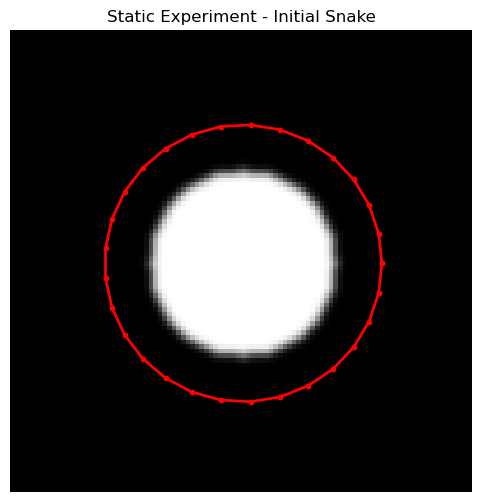
\includegraphics[width=0.5\linewidth]{output_1_simple.png}
    \caption{Static Image Iteration 1}
    \label{fig:enter-label}
\end{figure}
\begin{figure}[h!]
    \centering
    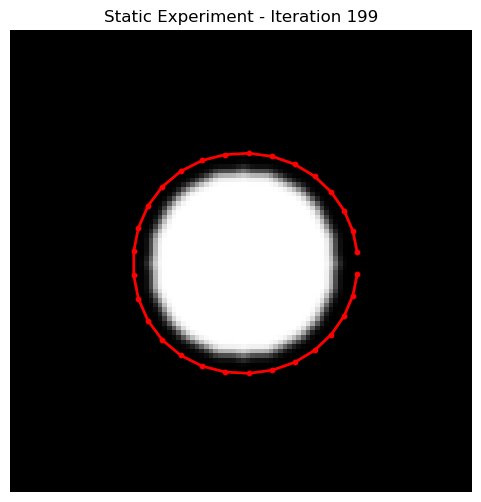
\includegraphics[width=0.5\linewidth]{output_122_simple.png}
    \caption{Static image Iteration 199}
    \label{fig:enter-label}
\end{figure}
\begin{figure}[h!]
    \centering
    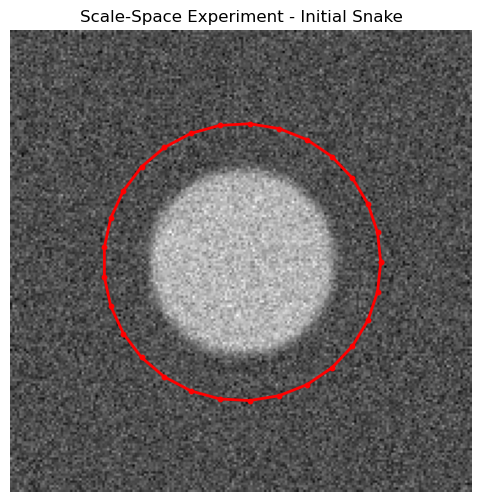
\includegraphics[width=0.5\linewidth]{output_122_sd.png}
    \caption{Scale-Space Iteration 1}
    \label{fig:enter-label}
\end{figure}
\begin{figure}[h!]
    \centering
    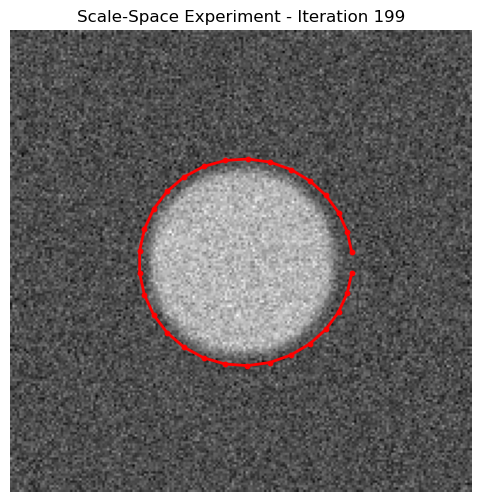
\includegraphics[width=0.5\linewidth]{output_122_simple_3244.png}
    \caption{Scale-Space Iteration 199}
    \label{fig:enter-label}
\end{figure}
{\small
\bibliographystyle{ieee_fullname}
\bibliography{egbib}
}

\end{document}